\documentclass{article}
\usepackage[utf8]{inputenc}
\usepackage{amsmath}
\usepackage{amssymb}
\usepackage{booktabs}
\usepackage{cancel}
\usepackage{enumitem}
\usepackage{graphicx}
\usepackage{mathtools}
\usepackage{mdframed}
\usepackage{multirow}
\usepackage{pgfgantt}
\usepackage{pdflscape}
\usepackage{appendix}
\usepackage{bbm}
\usepackage[margin=1in]{geometry}
\usepackage{biblatex} 
\addbibresource{library.bib}

\title{NE8 Lecture 2: The diffusion equation and power iteration}
\author{Paul Cosgrove}
\date{September 2022}

\begin{document}

\maketitle

\section{Deriving the diffusion equation}

Last time we ended with the monoenergetic, k-eigenvalue form of the transport equation with isotropic scattering:
\begin{equation}\label{eq:transport}
    \begin{split}
 \mathbf{\Omega}\cdot\nabla\psi + \Sigma_\mathrm{tr}\psi
    =\frac{1}{4\pi}\frac{\bar{\nu}\Sigma_\mathrm{f}}{ k_\mathrm{eff}}\phi + \frac{1}{4\pi}\Sigma_\mathrm{s}\phi\;\mathrm{.}
    \end{split}
\end{equation}
We are going to simplify this even further to obtain the neutron diffusion equation -- as well as being easy to solve analytically, eliminating two dimensions (by removing $\mathbf{\Omega}$, the neutron direction) means computers can also solve such equations with much less effort. 

Going forward, I'll revert the tr in $\Sigma_\mathrm{tr}$ to t in order to keep things clear. Just note that it actually pops up again in diffusion theory if we were to keep anisotropic scattering and in that case it would appear in our definition of the diffusion coefficient.

\subsection{1D transport equation}
To make the algebra easier, we're going to reduce the 3D Eq.~\eqref{eq:transport} to 1D. This will simplify the $\mathbf{\Omega}\cdot\nabla$ term to:
\begin{equation}
    \mathbf{\Omega}\cdot\nabla\psi(\mathbf{r},\mathbf{\Omega}) = \Omega_x \frac{\mathrm{d}}{\mathrm{d}x}\psi(x,\mathbf{\Omega})\;\mathrm{,}
\end{equation}
where $\Omega_x$ is the component/cosine of $\mathbf{\Omega}$ in the $x$-direction (which we often call $\mu$) and the derivatives in $y$ and $z$ will both go to zero. Now $\psi$ only depends on $\mu$, so we can integrate Eq.~\eqref{eq:transport} over the azimuthal angle (from 0 to $2\pi$) to get:
\begin{equation}\label{eq:transport_1D}
    \begin{split}
 \mu\frac{\mathrm{d}}{\mathrm{d}x}\psi(x,\mu) + \Sigma_\mathrm{t}\psi(x,\mu)
    =\frac{1}{2}\left[\frac{\bar{\nu}\Sigma_\mathrm{f}}{ k_\mathrm{eff}} + \Sigma_\mathrm{s}\right]\phi(x)\;\mathrm{.}
    \end{split}
\end{equation}
To make things clear, the relationship between fluxes is:
\begin{align}
\begin{split}
    \phi(x) = \int_{4\pi}\mathrm{d}\Omega\; \psi(x,\mathbf{\Omega}) = \int^{2\pi}_0 \mathrm{d}\varphi\int^{\pi}_{0}\mathrm{d}\theta\sin(\theta)\psi(x,[\varphi,\theta]) \\
    =\int^{2\pi}_0 \mathrm{d}\varphi\int^{1}_{-1}\mathrm{d}\left(\cos(\theta)\right)\psi(x,\cos(\theta))=2\pi \int^1_{-1}\mathrm{d}\mu\; \psi(x,\mu)
\end{split}
\end{align}

\subsection{Functional expansion}
One of the earliest ways of handling $\mathbf{\Omega}$ was not to discretise it, but to expand it using a convenient set of basis functions. We saw an example of this with scattering and Legendre polynomials. The basic concept is identical as to what is done with a Fourier series. If we have some function $f(x)$ over a given domain $D$ and some orthogonal basis of functions $p_n(x)$ which lie on the same domain, we can represent $f$ in term of $p_n$ as:
\begin{equation}\label{eq:expansion}
    f(x) = \sum^\infty_{n=0} f_n p_n(x)\;\mathrm{,}
\end{equation}
where $f_n$ is the component of $f$ corresponding to $p_n$. This component can be calculated as:
\begin{equation}\label{eq:component}
    f_n = \int_D \mathrm{d}x f(x) p_n(x)\;\mathrm{.}
\end{equation}
When trying to simplify or numerically solve an equation using functional expansion, we create a system of equations by applying Eq.~\eqref{eq:component} to the governing equation, to obtain an equation for each component -- if we have done things right, these should each be easier to solve than the original equation! We then truncate the expansion in Eq.~\eqref{eq:expansion} to some finite number of terms (giving us the number of equations to solve) and hope that they capture enough of the physics for our purposes.

\subsection{The P$_N$ method and diffusion}

It happens that for a variable like $\mathbf{\Omega}$ which is defined over the unit sphere, the natural set of basis functions are the spherical harmonics. Some of these are shown in Fig.~\ref{fig:SH}. They may be familiar from quantum mechanics or diffusion PDEs in spherical geometries.

\begin{figure}[h]
    \centering
    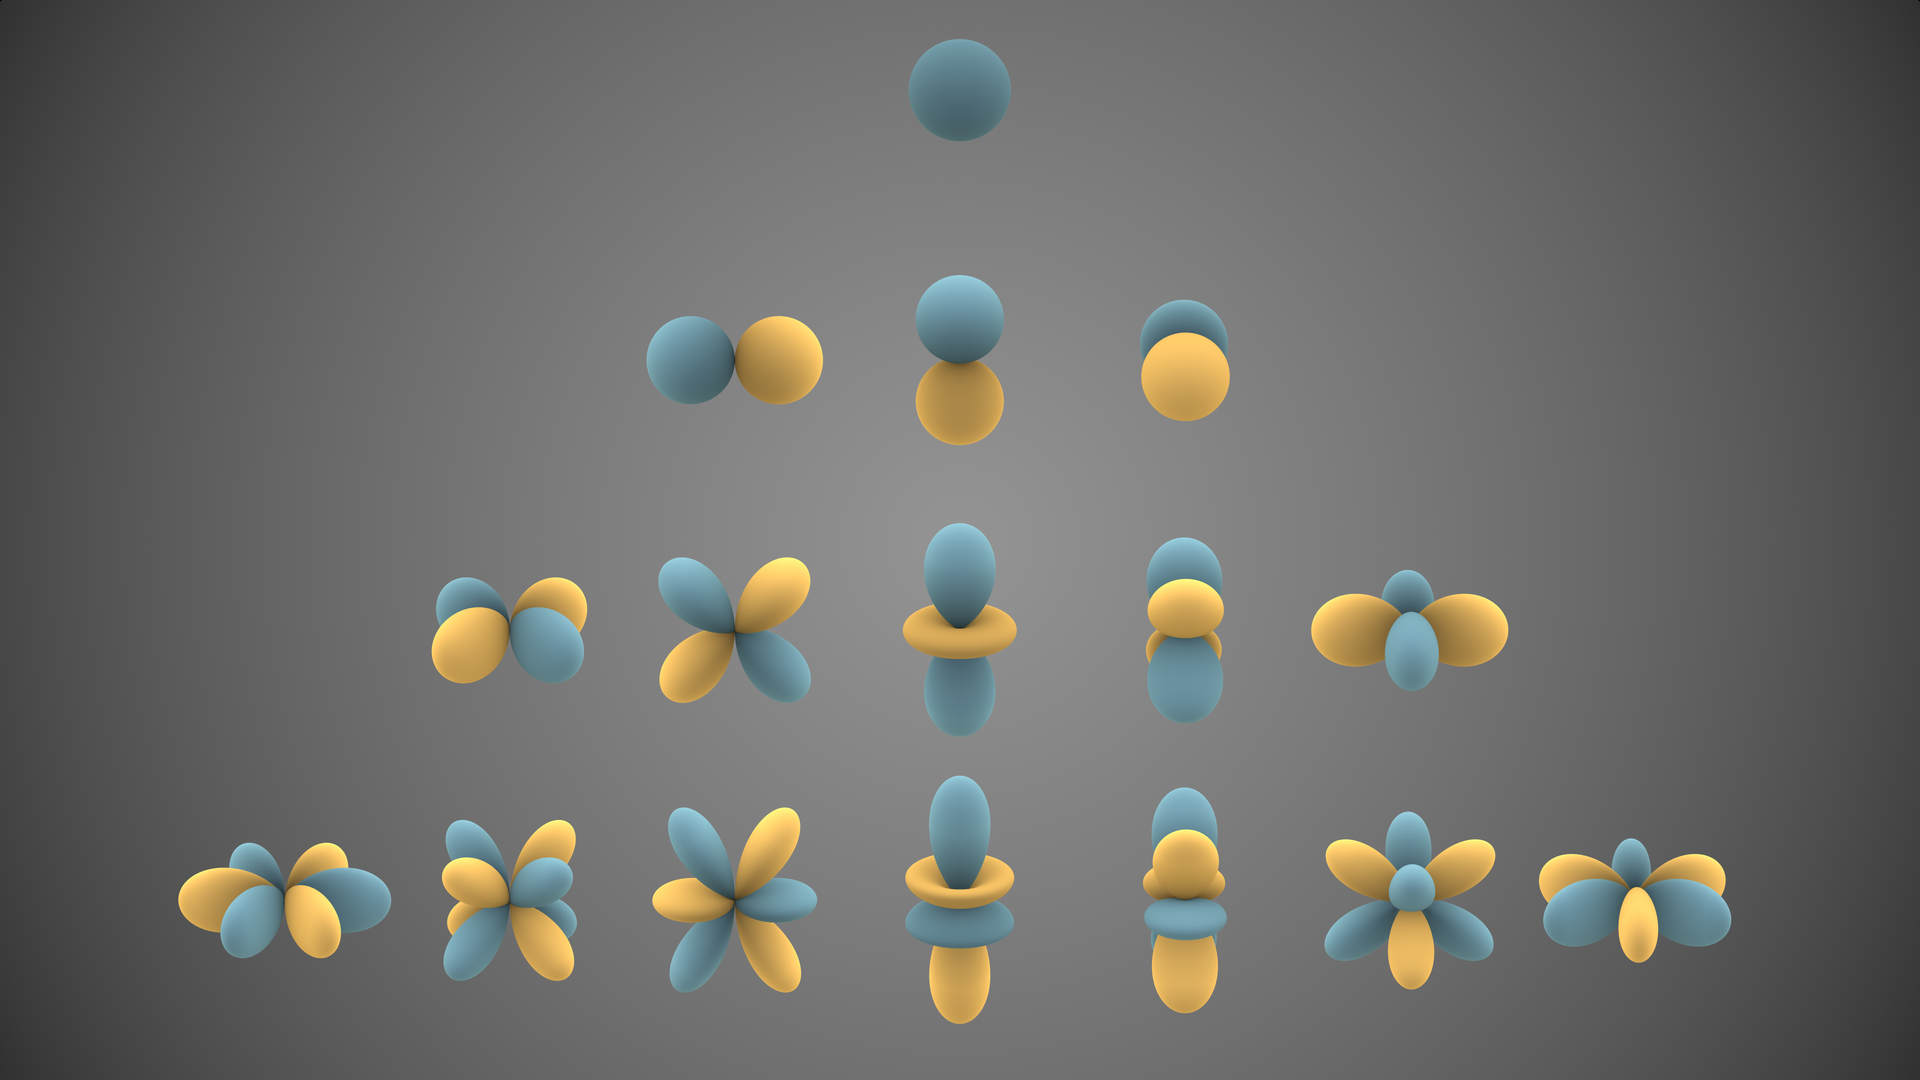
\includegraphics[width=0.6\linewidth]{./Spherical_Harmonics.png}
    \caption{The first few spherical harmonics (credit to Inigo.quilez on the spherical harmonics Wikipedia page)}
    \label{fig:SH}
\end{figure}

If we expand Eq.~\eqref{eq:transport} in spherical harmonics, we have what is known as the P$_N$ method, or simply the spherical harmonics method. In 1D, the spherical harmonics reduce to Legendre polynomials, making thing a bit clearer, so we'll expand the 1D transport equation (Eq.~\eqref{eq:transport_1D}) in Legendre polynomials instead. Appendix~\ref{appendix:legendre} gives some of the details of Legendre polynomials.

We begin expanding Eq.~\eqref{eq:transport_1D} by deciding the order, $N$, to which we will expand it. This means we can represent $\psi$ as:
\begin{equation}
    \psi(x,\mu)\approx\sum^N_{n=0}\frac{2n+1}{2}\phi_n(x)p_n(\mu)\;\mathrm{,}
\end{equation}
where $\phi_n$ is the $n$-th Legendre moment of the angular flux (making $\phi_0$ the standard scalar flux), and $(2n+1)/2$ is a normalising factor the polynomials require.
Then, for each Legendre polynomial, we multiply Eq.~\eqref{eq:transport_1D} by it and integrate with respect to $\mu$ from -1 to 1. 

In the general case this will result in a system of equations like:
\begin{equation}
    \begin{split}
 \frac{\mathrm{d}}{\mathrm{d}x}\phi_1(x) + \Sigma_\mathrm{t}\phi_0(x)
    =\left[\frac{\bar{\nu}\Sigma_\mathrm{f}}{ k_\mathrm{eff}} + \Sigma_\mathrm{s}\right]\phi_0(x)\mathrm{,}\;\;\mathrm{for }\; n = 0\;\mathrm{,}
    \end{split}
\end{equation}
\begin{equation}
    \begin{split}
 \frac{n}{2n+1}\frac{\mathrm{d}}{\mathrm{d}x}\phi_{n-1}(x) +  \frac{n+1}{2n+1}\frac{\mathrm{d}}{\mathrm{d}x}\phi_{n+1}(x) + \Sigma_\mathrm{t}\phi_n(x)
    =0\mathrm{,}\;\;\mathrm{for }\;n > 0\;\mathrm{.}
    \end{split}
\end{equation}
This gives us a system of simple equations in 1D slab geometry which can be solved very nicely. However, in general geometries this is not the case, making the P$_n$ equations \textbf{extremely} complicated to solve. This is because we would have to return to using spherical harmonics, making the number of equations to solve grow as $N^2$, which is not very practical! The equations also lose their simple form, making matters worse.

Where the P$_n$ method is most useful is as a theoretical justification for the diffusion equation. Let's say we expand only up to $N=1$, i.e., we assume that the angular flux is linearly anisotropic:
\begin{equation}
    \psi(\mu) \approx \frac{1}{2}\left(\phi_0 + 3\mu \phi_1\right)\;\mathrm{,}
\end{equation}
so $\phi_n = 0$ for $n>1$. Performing this expansion we obtain:
\begin{equation} \label{eq:P0}
    \begin{split}
 \frac{\mathrm{d}}{\mathrm{d}x}\phi_1(x) + \Sigma_\mathrm{t}\phi_0(x)
    =\left[\frac{\bar{\nu}\Sigma_\mathrm{f}}{ k_\mathrm{eff}} + \Sigma_\mathrm{s}\right]\phi_0(x)\;\mathrm{,}
    \end{split}
\end{equation}
\begin{equation}\label{eq:P1}
    \begin{split}
 \frac{1}{3}\frac{\mathrm{d}}{\mathrm{d}x}\phi_0(x) + \Sigma_\mathrm{t}\phi_1(x)
    =0\;\mathrm{.}
    \end{split}
\end{equation}
If we rearrange Eq.~\eqref{eq:P1}, we obtain something that looks quite a lot like Fick's law:
\begin{equation}\label{eq:Fick}
    \phi_1(x) = -\frac{1}{3\Sigma_\mathrm{t}}\frac{\mathrm{d}}{\mathrm{d}x}\phi_0(x)\;\mathrm{,}
\end{equation}
where we can equate $\phi_1 = J_x$ and $\frac{1}{3\Sigma_\mathrm{t}}=D$ (or $\frac{1}{3\Sigma_\mathrm{tr}}$ if we were being more rigorous). 
 Inserting Eq.~\eqref{eq:Fick} into Eq.~\eqref{eq:P0} gives our familiar diffusion equation:
\begin{equation}
    -\frac{\mathrm{d}}{\mathrm{d}x}D\frac{\mathrm{d}}{\mathrm{d}x}\phi_0(x) + \left[\Sigma_\mathrm{a} - \frac{\nu\Sigma_\mathrm{f}}{k_\mathrm{eff}}\right]\phi_0(x) = 0\;\mathrm{.}
\end{equation}
You might think that if truncating at $N=1$ is useful, then it might be interesting to truncate even sooner at $N=0$. You could try it and see what happens...

\subsection{Simplified P$_N$}
I should also add that while the P$_N$ method is not very popular, it has a cousin known as the Simplified P$_N$ method (or SP$_N$) which is much more practical -- if a bit less general. 

The logic behind SP$_N$ goes: `P$_N$ is really nice in 1D slab geometry. What if it looked like that for every geometry? Well, that just means replacing $\frac{\mathrm{d}}{\mathrm{d}x}$ with $\nabla$ everywhere!' Lo and behold, the results it produces aren't too bad -- often the method is referred to as being partway between diffusion and transport, or diffusion with some extra transport effects. An SP$_N$ solver can also be quite easily written when starting with a diffusion solver without making any major changes. 

While it was originally stumbled upon in exactly this irrigorous way, it has since been justified with more careful analysis. A great description and discussion of the method can be found in \cite{McClarren} for those interested.

\subsection{Limitations of neutron diffusion}

The preceding was a rough `derivation' of the neutron diffusion equation, but there are several others. Some of these are better in that they make more clear which approximations are being made and so when diffusion is or isn't applicable.

The most rigorous of these derivations is by `asymptotic analysis'. It has not been included here because it's much more mathematically involved than we have time to discuss, but I recommend looking it up in your own time if you are curious. A very accessible derivation is given in \cite{Adams}. It starts by saying `what if neutron absorption is small, neutron sources are weak, and the system is optically thick (neutrons travel short distances between collisions)'. These can all be written mathematically as:
\begin{equation}\label{eq:transport_asymp}
    \begin{split}
 \mu\frac{\mathrm{d}}{\mathrm{d}x}\psi(x,\mu) + \frac{\Sigma_\mathrm{t}}{\epsilon}\psi(x,\mu)
    =\frac{1}{2} \left(\frac{\Sigma_\mathrm{t}}{\epsilon}-\epsilon\Sigma_\mathrm{a}\right)\phi(x)+\epsilon \frac{Q(x)}{2}\;\mathrm{,}
    \end{split}
\end{equation}
where $Q$ is a generic isotropic neutron source (replacing fission to keep things neat), the scattering cross section has been rewritten as total minus absorption, and $\epsilon$ is a small dimensionless parameter ($\epsilon <<1$) used to scale the different terms of the equation and show their relative magnitudes.

Following this equation through, one can obtain the diffusion equation. The important point here is that this implies diffusion is a valid approximation when:
\begin{itemize}
    \item Neutron sources are small
    \item Scattering greatly dominates absorption
    \item Neutron flux varies `slowly' in space and angle -- usually far from material boundaries
    \item The system is large in terms of neutron mean free paths: $\Sigma_\mathrm{t}L >> 1$, where $L$ is a characteristic length of the system
\end{itemize}

\section{Power iteration -- solving eigenvalue problems}

Whether we try to solve a transport or diffusion equation, we end up with an eigenvalue problem. Eigenvalue problems should be familiar from linear algebra: if we have a matrix $\mathbf{A}$ which has an eigenvector $y$, they will satisfy the following equation:
\begin{equation}
    \mathbf{A}y = \lambda y\;\mathrm{,}
\end{equation}
where $\lambda$ is a scalar known as the eigenvalue. Often we come across a generalised eigenvalue problem, which looks like:
\begin{equation}
    \mathbf{A}y = \lambda \mathbf{B}y\;\mathrm{,}
\end{equation}
where $\mathbf{B}$ is another matrix -- this can be transformed back into an eigenvalue problem by left-multiplying by $\mathbf{B}^{-1}$ provided $\mathbf{B}$ is invertible.

Compare these with the diffusion equation, which can be written as:
\begin{equation}\label{eq:diffusion_operators}
    \left[-\frac{\mathrm{d}}{\mathrm{d}x}D\frac{\mathrm{d}}{\mathrm{d}x} + \Sigma_\mathrm{a}\right] \phi(x) = \frac{\nu\Sigma_\mathrm{f}}{k_\mathrm{eff}}\phi(x)\;\mathrm{.}
\end{equation}
As can be seen, this is clearly a generalised eigenvalue problem if we say that our continuous function $\phi(x)$ is the eigenvector, our continuous diffusion plus absorption and fission operators are the matrices $\mathbf{A}$ and $\mathbf{B}$, and $1/k_\mathrm{eff}$ is our eigenvalue. Many areas in physics and mathematics are concerned with solving eigenvalue problems and the approaches taken in neutronics are similar to those used elsewhere.

\subsection{Classic power iteration}
One of the simplest but most robust approaches is power iteration. Power iteration is a means of finding the dominant eigenvalue and eigenvector of a matrix, provided the matrix is \textbf{diagonalisable}. If unfamiliar, you needn't worry too much about the definition, but ultimately it means we have a square matrix of dimension $n$ with $n$ distinct eigenvectors. These eigenvectors form a basis, i.e., for any generic vector $y$, we can write it in terms of the eigenvectors, $x_i$, of the matrix as:
\begin{equation}
    y = a_1 x_1 + a_2 x_2 +\ldots + a_n x_n\;\mathrm{,}
\end{equation}
where $a_i$ are the components of $y$ in the direction of the eigenvector $x_i$. We also assume that for its eigenvalues, $\lambda_i$, there is one eigenvalue which is larger than all other others -- we will call it $\lambda_1$.

Power iteration searches for the dominant eigenpair ($x_1,\lambda_1$) of matrix $\mathbf{A}$. It does this beginning with a guess vector, $y^{(0)}$. This vector is multiplied by $\mathbf{A}$ to give $y^{(1)}$. This operation can be written as:
\begin{equation}
    y^{(1)} = \mathbf{A}y^{(0)} = \mathbf{A}\left[a_1 x_1 + a_2 x_2 +\ldots + a_n x_n\right]\mathrm{.}
\end{equation}
We can see that the matrix $\mathbf{A}$ is operating on its eigenvectors, giving:
\begin{equation}
    y^{(1)} = \lambda_1 a_1 x_1 + \lambda_2 a_2 x_2 + \ldots \lambda_n a_n x_n\;\mathrm{.}
\end{equation}
If we apply this operation $m$ times we get:
\begin{equation}
    y^{(m)} = \mathbf{A}^m y^{(0)} = \lambda^m_1 a_1 x_1 + \lambda^m_2 a_2 x_2 + \ldots \lambda^m_n a_n x_n\;\mathrm{,}
\end{equation}
which can be rewritten as:
\begin{equation}\label{eq:power_eigen}
    y^{(m)} = \lambda^m_1 \left(a_1 x_1 + \left(\frac{\lambda_2}{\lambda_1}\right)^m a_2 x_2 + \ldots \left(\frac{\lambda_n}{\lambda_1}\right)^m  a_n x_n\right)\;\mathrm{.}
\end{equation}
As $\lambda_1$ is the largest eigenvalue, the ratio $\frac{\lambda_i}{\lambda_1}$ must always be less than 1. Therefore, as $m\rightarrow\infty$, the contributions of higher eigenvectors (in relative terms) approach zero, leaving only the fundamental eigenvector. To ensure numerical stability , there is usually a normalisation of the resulting vector after multiplication by $\mathbf{A}$ such that power iteration can be written simply as the recurrence relation:
\begin{equation}
    y^{(m+1)}=\frac{\mathbf{A}y^{(m)}}{||\mathbf{A}y^{(m)}||}\;\mathrm{,}
\end{equation}
where $||\cdot||$ denotes taking the norm of a vector. For a sufficiently large value of $m$, the eigenvalue can be estimated as:
\begin{equation}
    \lambda_{1,m} = \frac{||\mathbf{A}y^{(m)}||}{||y^{(m)}||}\;\mathrm{.}
\end{equation}
This iteration is usually terminated when the change in either the eigenvalue or the eigenvector are sufficiently small as decided by some user-specified criterion:
\begin{equation}
    \frac{||y^{(m+1)} - y^{(m)}||}{||y^{(m+1)}||}<\epsilon_y\;\mathrm{,}
\end{equation}
\begin{equation}
    \frac{|\lambda_{1,m+1} - \lambda_{1,m}|}{|\lambda_{1,m+1}|}<\epsilon_\lambda\;\mathrm{.}
\end{equation}
Power iteration is a simple algorithm and while robust, is often known as being slow. The speed of power iteration's convergence is problem dependent. \textbf{Based on Eq.}~\eqref{eq:power_eigen}\textbf{, what might control the rate of convergence?} There are many methods of accelerating power iteration, but these will be left for another time.

\subsection{Power iteration in neutron diffusion}

The application of power iteration to neutronics is nearly identical as above. We have a slightly extra step to go through in the general case because, while the eigenvector we care about is the \textbf{fission source}, $F$, the equations of neutronics are most naturally solved for the flux $\phi$. This is because neutron scattering is also present if we were solving a multi-group diffusion problem (or any transport problem). We will ignore this for now, but it will reappear when we consider transport problems.

Our aim is to transform Eq.~\eqref{eq:diffusion_operators} into  something that can be solved using power iteration. We make the following definition:
\begin{equation}
    \mathbf{L} = \left[-\frac{\mathrm{d}}{\mathrm{d}x}D\frac{\mathrm{d}}{\mathrm{d}x} + \Sigma_\mathrm{a}\right]\;\mathrm{,}
\end{equation}
where $\mathbf{L}$ is a matrix which represents some spatial discretisation of the continuous diffusion plus absorption terms. We also say that $\nu\Sigma_\mathrm{f}$ is discretised to give a matrix (which we will write identically as before). This allows us to rewrite the diffusion equation as:
\begin{equation}
    \mathbf{L}^{-1}\nu\Sigma_\mathrm{f}\phi = k\phi\;\mathrm{,}
\end{equation}
which is exactly the standard eigenvalue problem. Finally, if we choose some guess flux vector, $\phi^{(0)}$, and some guess eigenvalue, $k_0$, we can perform power iteration. We do this by calculating the fission source (normalised by the estimate of the eigenvalue), inverting the diffusion plus absorption matrix to obtain a new flux estimate, and then using this to calculate a new eigenvalue. In equation form, this can be written as:
\begin{equation}
    \phi^{(m+1)}=\mathbf{L}^{-1}\frac{1}{k^{(m)}}\nu\Sigma_\mathrm{f}\phi^{(m)}\;\mathrm{,}
\end{equation}
\begin{equation}
    k^{(m+1)} = k^{(m)} \frac{\int \mathrm{d}x\; \nu\Sigma_\mathrm{f}\phi^{(m+1)}}{\int \mathrm{d}x\; \nu\Sigma_\mathrm{f}\phi^{(m)}}\;\mathrm{.}
\end{equation}
These equations (and some termination criterion) are sufficient to perform power iteration. You will use this for the upcoming piece of coursework.

Note that this is still quite simplified. In practical diffusion problems the matrices we form will be over \textbf{space and energy}. The principle would be the same, but we would also account for neutron scattering from one group to another and for fission contributions in all different energy groups. An example of the sort of matrix that is constructed, even for a small 4$\times$4 problem, is shown in Fig.~\ref{fig:matrix}.

\begin{figure}[h]
    \centering
    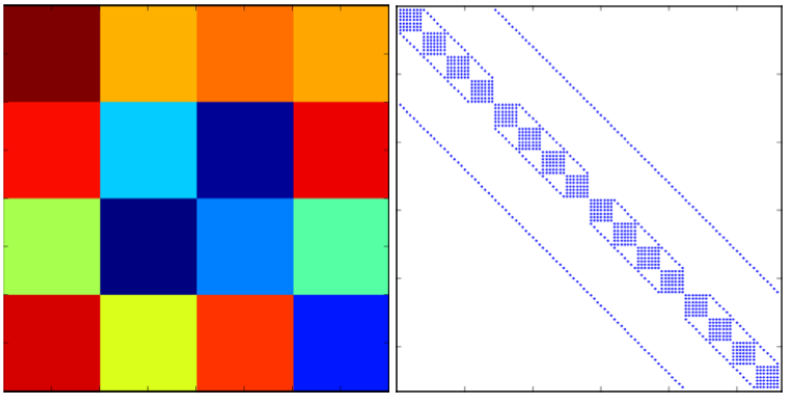
\includegraphics[width=0.6\linewidth]{./matrix.png}
    \caption{7-group 2D diffusion problem mesh (left) and matrix sparsity plot (right) \cite{openmoc}}
    \label{fig:matrix}
\end{figure}

Handling large matrices such as these efficiently often means we cannot easily use direct methods of matrix inversion. Instead, we take advantage of the sparsity of the matrix and use iterative methods to invert it. This is much cheaper since, for a sufficiently sparse matrix, there will be fewer operations required to repeatedly do sparse matrix vector multiplication than to perform one of the direct matrix inversion algorithms. For example, in MATLAB one can identify a matrix as sparse by saying {\fontfamily{qcr}\selectfont A = sparse(A)} and then fast iterative methods will be used for all operations involving that matrix afterwards.

\printbibliography

\appendix

\section{Legendre polynomials}\label{appendix:legendre}

Legendre polynomials, $p_n(x)$ are a series of polynomial functions defined on the domain $x\in[-1,1]$. Their orthogonality relationship is:
\begin{equation}
    \int^1_{-1}\mathrm{d}x\; p_n(x) p_m(x) = \frac{2}{2n+1}\delta_{nm}\;\mathrm{,}
\end{equation}
where $\delta_{nm}$ is the Kronecker delta function, equal to 1 if $n=m$ and equal to 0 otherwise. A function can be expressed as a sum of Legendre polynomials as:
\begin{equation}
    f(x) = \sum^\infty_{n=0}\frac{2n+1}{2}f_n p_n(x)\;\mathrm{,}
\end{equation}
where the component of function $f(x)$ corresponding to the $n$-th Legendre polynomial is given by:
\begin{equation}
    f_n = \int^1_{-1}\mathrm{d}x\; f(x) p_n(x)\;\mathrm{.}
\end{equation}

The first few Legendre polynomials are given in Table~\ref{table:legendre}.

\begin{table}[h!]
\centering
\caption{The first five Legendre polynomials}
\renewcommand{\arraystretch}{2}
\begin{tabular}{|c|c|}
\hline
Order $n$ & Legendre polynomial $p_n(x)$            \\ \hline
0         & 1                                       \\ \hline
1         & $x$                                     \\ \hline
2         & $\frac{1}{2}\left(3x^2-1\right)$        \\ \hline
3         & $\frac{1}{2}\left(5x^3-3x\right)$       \\ \hline
4         & $\frac{1}{8}\left(35x^4-30x^2+3\right)$ \\ \hline
\end{tabular}\label{table:legendre}
\renewcommand{\arraystretch}{1}
\end{table}

\end{document}
